\chapter{Implementacja}
\thispagestyle{chapterBeginStyle}

\section{Opis komponentów i ich połączeń}
    W programie implementującycm algorytm będący obiektem badań można wyróżnić 3 główne komponenty:
    \begin{itemize}
        \item \textbf{Algorytm} zaimplementowany w języku programowania \textbf{PROLOG}
        \item \textbf{Generator grafów} zaimplementowany w formie modułu w języku programowania \textbf{Python}
        \item \textbf{Warstwa graficzna} (GUI) zaimplementowana w języku programowania \textbf{Python} przy użyciu bibloteki \textbf{Tkinter}
    \end{itemize}
    Naistostniejszą z perspektywy użytkownika jest \textbf{Warstwa graficzna}. Jest to program, którego uruchomienie pozwala na 
    interakcję z utworzonym narzędziem w przyjazny dla użytkownika sposób. Istnieje również możliwość uruchomienia algorytmu z pominięciem 
    warstwy graficznej, o czym można dowiedzieć się więcej w sekcji \ref{CommandLine}.
    Z wyświetlonego menu użytkownik może wybrać przykładowe, wcześniej spreparowane światy, zdefiniować swój stan początkowy oraz cel (w niektórych 
    światach cel jest intuicyjny, więc jego definicja nie jest od użytkownika wymagana) i uruchomić algorytm. Wynikiem działania programu jest 
    plan, który wyświetlony jest w formie tekstowej z opisem na kroki oraz dwa grafy: graf pełen (zawierający wszystkie składowe opisane 
    w \ref{GRAPHPLANRozdzial}) oraz graf uproszczony, który zawiera jedynie niezbędne stany oraz akcje wymagane do zrozumienia wygenerowanego planu.
    Poniższy schemat klarownie przedstawia relacje między komponentami w trakcie działania programu:
    \begin{figure}[H]
        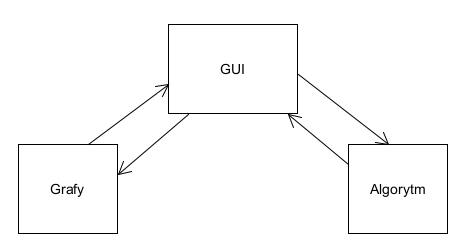
\includegraphics[scale=0.5]{zaleznosci}
        \centering
        \caption{Zależności między komponentami}
    \end{figure}
    Główna jednostką sterującą jest warstwa graficzna. W momencie naciśnięcia przez użytkownika odpowiedniego przycisku generującego rozwiązania, warstwa 
    graficzna zbiera wszystkie niezbędne informacje: w jakim świecie użytkownik pracuje, w jaki sposób zdefiniował warunki początkowe, oraz jakie cele 
    chce on uzyskać. Następnie obrobione informacje przesyłane są do algorytmu, który poza wygenerowaniem planu, do pliku tekstowego wypisuje 
    stany, akcje oraz mutexy dla każdej z warstw. Następnie algorytm przesyła swoją odpowiedź do GUI, 
    który wysyła żadanie wygenerowania grafów do odpowiednich komponentów odpowiedzialnych za ich 
    generowanie. W skład komponentu "Grafy" wchodzą dwie klasy, przy czym każda z nim generuje unikalny graf.

\section{Implementacja algorytmu}
    Algorytm \textbf{GRAPHPLAN} został zaimplementowany w języku programowania PROLOG. Poniższe diagramy przedstawiają proces  
    generowania pojedynczego planu.
    \begin{figure}[H]
        \label{PetlaGlowna}
        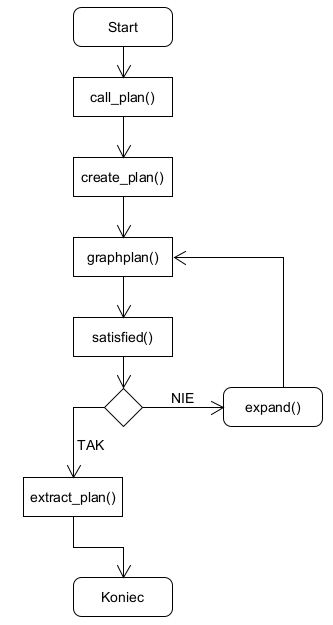
\includegraphics[scale=0.75]{GRAPHPLAN_petla_glowna}
        \centering
        \caption{Główna pętla algorytmu}
    \end{figure}

    \begin{definition}
        \label{Predykat}
        \textbf{Klauzula} -- przedstawiona informacja o świecie
    \end{definition}

    \begin{definition}
        \label{Fakt}
        \textbf{Fakt} -- informacja o świecie, która jest zawsze prawdziwa
    \end{definition}

    \begin{definition}
        \label{Regula}
        \textbf{Reguła} -- informacje, które są prawdziwe, po spełnieniu pewnych warunków
    \end{definition}

    \begin{definition}
        \label{Predykat}
        \textbf{Predykat} -- sposób wyrażania warunków w programowaniu w logice
    \end{definition}


    Przed rozpoczęciem omawiania struktury programu wprowadzono podstawowe definicje stosowane w programowaniu w logice. Przykładem klauzuli jest 
    zdanie $kobieta(anna).$ informujące program o tym, iż Anna jest kobietą. Ze względu na sposób reprezentacji danych w języku programowania PROLOG, 
    wszystkie stałe określane są małymi literami, gdyż ciągi znaków zaczynające się wielką literą zarezerwowane są dla \textit{zmiennych}. Należy 
    również zwrócić uwagę na wykorzystanie znaku przystankowego w postaci kropki (\textbf{.}), przedstawiający koniec przekazywanej informacji. 
    $kobieta(anna).$ również jest przykładem jednoargumentowego predykatu. Predykaty jednoargumentowe często określanę są mianem \textit{własności}.
    Predykaty o większej liczbie argumentów często nazywane są \textit{relacjami}. W Prologowej nomenklaturze predykaty zapisuję się zgodnie 
    z następującą strukturą: \textit{X/Y}, gdzie \textit{X} oznacza nazwę relacji (nagłówek), a \textit{Y} liczbę argumentów przyjmowaną przez 
    opisywany predykat. Zgodnie z powyższym zapis $kobieta/1$ oznacza, iż relacja kobieta przyjmuje jeden argument.
    Zdanie $kolor(brązowy).$ jest przykładem faktu, czyli zdania zawsze prawdziwego. Fakty różnią się od reguł tym, iż reguły nie muszą być zawsze prawdziwe \cite{PROLOG}.
    W sekcji \ref{DefinicjeSwiata} wprowadzono przykład reguły, wraz z opisem jej struktury.

    Założeniem działania algorytmu jest poprawne zdefiniowanie warunków początkowych oraz celów, przy użyciu wcześniej spreparowanych przez użytkownika 
    relacji. Ponadto zbiór akcji również musi zostać bezpośrednio utworzony przez użytkownika, algorytm w trakcie działania nie dokonuje żadnego 
    sprawdzenia zgodności wprowadzonych danych. Z tego powodu warstwa graficzna programu udostępnia tylko część środowisk, które zostały opisane przez 
    autora pracy zgodnie z wytycznymi języka opisu STRIPS.

    Predykat o nazwie $call\_plan/2$ odpowiada za utworzenie pliku tekstowego (nazwa pliku: \textit{output.txt}) oraz przekierowanie strumienia danych 
    do ustalonego pliku. Następnie pobiera stan świata, które zdefiniowany jest w formie faktu \textit{inital\_state/1}, który przyjmuje jeden argument
    w formie listy zawierającej wszystkie stany początkowe. Następnie dochodzi do uruchomienia predykatu $create\_plan/3$, który przyjmuje jako dane
    wejściowe początkowy stan oraz wymagany cel, a wynikiem jego działania jest utworzony plan. W tym predykacie, z pomocą predykatu $findall/3$,
    odbywa się nadanie wszystkim stanom początkowym indykatora jeden, gdyż wszystkie z tych stanów są prawdziwe w przedstawionym świecie. 
    Następnie dochodzi do wykreowania pierwszego zbioru akcji przy pomocy wbudowanego predykatu $setof/3$. Po wykreowaniu odpowiednich zbiorów 
    dochodzi do uruchomienia predykatu $graphplan/4$ - głównej pętli programu.

    \begin{listing}[H]
        \begin{minted}{prolog}
            % call_plan(+Goals,-Plan)
            call_plan(Goals,Plan) :-
                tell('outputs/output.txt'),
                inital_state(S),
                create_plan(S,Goals,Plan),
                write("Plan: "), writeln(Plan),
                told.
        \end{minted}
        \caption{Implementacja predykatu call\_plan/2}
    \end{listing}

    \begin{listing}[H]
        \begin{minted}{prolog}
            % create_plan(+StartState,+Goals,-Plan)
            create_plan(StartState, Goals, Plan) :-
                findall(State/1, member(State,StartState),StartLevel),
                setof(action(Action, Precondition, Effects), 
                (effects(Action,Effects),preconditions(Action,Precondition)),
                AllActions),
                write("StartLevel: "), write(StartLevel), nl,
                graphplan([StartLevel], Goals, Plan, AllActions).
    \end{minted}
    \caption{Implementacja predykatu create\_plan/2}
    \end{listing}

    Działanie predykatu $graphplan/4$ można podzielić na dwa etapy. W pierwszym etapie sprawdzany jest warunek konieczny utworzenia grafu- 
    obecność wszystkich stanów ze zbioru celów na aktualnym poziomie stanów. Dokonywane jest to przy pomocy predykatu $satisfied/2$, który 
    iteruje po każdym celu z listy celów i dokonuje sprawdzenia wskazanego warunku. Dodatkowo rzeczona klauzula ustala, czy indykator każdego z 
    celów jest większy od zera, czyli czy jest możliwość jego wykonania na danym poziomie stanów. Jeśli powyższe warunki są spełnione dla każdegu celu, 
    algorytm przechodzi do predykatu $extract\_plan/2$, który na podstawie aktualnego poziomu stanów 
    podejmuję próbę generowania odpowiedniego plan. 
    
    \begin{listing}[H]
        \begin{minted}{prolog}
            % graphplan(+GraphPlan,+Goals,+AllActions,-Plan)
            graphplan([StateLevel | GraphPlan], Goals, AllActions,Plan) :-
                satisfied(StateLevel, Goals),
                extract_plan([StateLevel | GraphPlan], Plan)
                ;
                expand(StateLevel, ActionLevel, NewStateLevel, AllActions),
                graphplan([NewStateLevel, ActionLevel, StateLevel | GraphPlan], 
                Goals, AllActions, Plan).
    \end{minted}
    \caption{Implementacja predykatu graphplan/4}
    \end{listing}
    
    \begin{listing}[H]
        \begin{minted}{prolog}
            % satisfied(+StateLevel, +Goals)
            satisfied(_,[]).

            satisfied(StateLevel, [G | Goals]) :-
                member(G/IG, StateLevel),
                IG #> 0,
                satisfied(StateLevel, Goals).
    \end{minted}
    \caption{Kod źródłowy implementacji predykatu satisfied/2}
    \end{listing}

    \begin{listing}[H]
        \begin{minted}{prolog}
            % extract_plan(+Graph,-Plan)
            extract_plan([_],[]).

            extract_plan([ChosenStates,ActionLevel | RestOfGraph], Plan) :-
                collect_vars(ActionLevel, AVars),
                labeling([],AVars),
                findall(A, (member(A/1,ActionLevel)),ChosenActions),
                extract_plan(RestOfGraph, RestOfPlan),
                write("ChosenActions: "), write(ChosenActions),nl,
                write("ChosenStates: "), writeln(ChosenStates),
                append(RestOfPlan, [ChosenActions], Plan).
    \end{minted}
    \caption{Implementacja predykatu extract\_plan/2}
    \end{listing}

    W przeciwnym wypadku  algorytm przechodzi do drugiej części, 
    w której dochodzi do rozszerzenia grafu planującego o kolejne warstwy przy pomocy predykatu $expand/4$. 
    Predykat $expand/4$ ma za zadanie rozszerzyć graf o kolejną warstwę. Wykonuje to korzystając z dwóch predykatów, których nazewnictwo w pełni 
    odpowiada funkcjonalności, jakie implementują. Są to- $add\_action/6$, którego zadaniem jest generowanie oraz dodawanie akcji do poziomu akcji 
    danej warstwy oraz $mutex\_state/1$ oraz $mutex\_action/2$, odpowiedzialne za tworzenie relacji wzajemnie wykluczających między stanami jak i akcjami.
    W ramach predykatu $add\_action/6$ realizowany jest również predykat $add\_effects/4$, który dla każdej akcji dodaje jej efekty do przyszłego 
    poziomu stanów.
    
    
    \begin{listing}[H]
        \begin{minted}{prolog}
        % expand(+StateLevel, -ActionLevel, -NextStateLevel, +AllActions)
            expand(StateLevel, ActionLevel, NextStateLevel, AllActions) :-
                add_actions(StateLevel, AllActions, [], NewActionLevel, [], NewNextState),
                findall(action(zostan(P),[P],[P]),member(P/_,StateLevel),PersistActs),
                add_actions(StateLevel, PersistActs, NewActionLevel, 
                ActionLevel, NewNextState, NextStateLevel),
                mutex_action(ActionLevel,NextStateLevel), 
                mutex_list(NextStateLevel),
                write("ActionLevel: "), write(ActionLevel),nl,
                write("StateLevel: "), write(NextStateLevel), nl.
    \end{minted}
    \caption{Implementacja predykatu expand/4}
    \end{listing}

    Predykat $write/1$ wykorzystywany jest wyłącznie w celu umieszczenia odpowiednich informacji o poziomie stanów oraz o poziomie akcji w pliku
    tekstowym, ktory następnie wykorzystywany jest podczas generowania odpowiednich grafów.

    \begin{listing}[H]
        \begin{minted}{prolog}
            %add_actions(+StateLevel,+Action,+PreviousActionLevel,
            -NewActionLevel,+PreviousStateLevel,-NewStateLevel)
            add_actions(_,[],ActionLevel, ActionLevel, NextStateLevel, NextStateLevel).

            add_actions(StateLevel, [action(A,Precondition,Effects) | Acts], 
            ActLev0, ActLev, NextLev0, NextLev) :-
                IA in 0..1, 
                includes(StateLevel, Precondition, IA),
                add_effects(IA, Effects, NextLev0, NextLev1), !, 
                write("A: "), write(A), nl,
                write("Precondition: "), write(Precondition), nl,
                write("Effects: "), write(Effects), nl,
                add_actions(StateLevel, Acts, [A/IA | ActLev0], ActLev, NextLev1, NextLev)
                ;
                add_actions(StateLevel, Acts, ActLev0, ActLev, NextLev0, NextLev).
    \end{minted}
    \caption{Implementacja predykatu add\_actions/6}
    \end{listing}

    Przy implementacji predykatu $add\_actions/6$ należy zwrócić uwagę na wykorzystanie programowania ograniczeń w formie zmiennej \textbf{IA}, 
    która przyjmuje wartość ze zbioru $\{0,1\}$, gdyż akcja może, ale nie musi być realizowana na danym poziomie akcji. Dodatkowo rzeczony 
    predykat korzysta z predykatu $includes/3$, który dodaje warunek na wartość przyjmowaną przez identyfikator akcji- nie może być on większy 
    niż identyfikator warunków zajścia. Należy to interpetować w następujący sposób: jeśli którykolwiek z warunków początkowych miałby w danym 
    poziomie wartość równą 0 (czyli byłby nieprawdziwy), wtedy dana akcja nie może znajdować się w planie na wskazanym poziomie, natomiast 
    prawdziwość wszystkich warunków (czyli identyfiaktora równego 1 dla każdego warunku), powoduje iż akcja znajdzie się w zbiorze potencjalnych
    akcji do wykonania na wskazanym poziomie.

    \begin{listing}[H]
        \begin{minted}{prolog}
            % includes(+StateLevel, +Preconditions, +Indykator)
            includes(_,[],_).

            includes(StateLevel, [P|Ps],IA) :-
                member(P/I, StateLevel),
                IA #=< I,
                includes(StateLevel, Ps, IA).
    \end{minted}
    \end{listing}

    \begin{listing}[H]
        \begin{minted}{prolog}
            %add_effects(+Indykator,+PreviousStateLevel,-NextStateLevel)
            add_effects(_,[],StateLevel,StateLevel).

            add_effects(IA, [P | Ps], StateLev0, ExpandedState) :-
                (remove(P/IP,StateLev0,StateLev1),!,
                NewIP #= IP+IA,
                StateLevel = [P/NewIP | StateLev1]
                ;
                StateLevel = [P/IA | StateLev0], !
                ),
                add_effects(IA, Ps, StateLevel, ExpandedState).
    \end{minted}
    \caption{Implementacja predykatu add\_effects/4}
    \end{listing}
    
    
    Następnie, w celu zachowania spójności, dla utworzonych zbiorów 
    generowane są relacje wzajemnego wykluczania określone mianem \textit{mutex'ów}. Mechanizm mutex'ów implementowany jest przy pomocy dwóch predykatów:
    \begin{itemize}
        \item \textbf{mutex\_state/1} - predykat odpowiedzialny za ustalenie, które stany znajdują się w relacji wykluczającej na wskazanym 
        poziomie generowania planu
        \item \textbf{mutex\_action/2} - predykat odpowiedzialny za ustalenie, które akcje znajdują się w relacji wykluczającej na wskazanym
        poziomie generowania planu. Dodatkową funkcjonalnością rzeczone predykatu jest ustalenie mutex'ów między efektami akcji, które 
        nie zawsze muszą być objęte definicjami wprowadzonymi w ramach \textbf{mutex\_state/1}.
    \end{itemize}

    Działanie predykatów jest bardzo zbliżone z tą różnicą, iż operują na innych obiektach. Schemat działania prezentuje się w sposób następujący:
    \begin{enumerate}
        \item Ustal element ze zbioru stanów
        \item Następnie dobierz do pary każdy z pozostałych elementów poziomu stanów i sprawdź, czy ów stany wykluczają się wzajemnie
        \item Wróć do pierwszego kroku, jako element ustalając następny obiekt wchodzący w skład listy stanów
    \end{enumerate}

    Powyższy opis został zaprezentowant z perspektywy predykatu \textbf{mutex\_state/1}. Dla predykatu \textbf{mutex\_action/2} jedyną różnicą jest 
    dodatnie ostatniego kroku, w którym wszystkie efekty wskazanych akcji zostają ze sobą połączone relacją wzajemnie wykluczającą. Determinowane 
    jest to uniknięciem sytuacji określanej w sekcji \ref{WzajemneWykluczanieRozdzial} jako \textbf{niespójny efekt}.

    \begin{listing}[H]
        \begin{minted}{prolog}
            %mutex_state(StateLevel)
            mutex_state([]).

            mutex_state([P | Ps]) :-
            mutex_single(P,Ps),
            mutex_state(Ps).
        \end{minted}
    \caption{Implementacja predykatu mutex\_state/1}
    \end{listing}

    \begin{listing}[H]
        \begin{minted}{prolog}
            %mutex_single(+State,+StateLevel)
            mutex_single(_,[]).

            mutex_single(P/I, [P1/I1 | Rest]) :-
                ( mutex(P,P1), !, I*I1 #= 0
                ;
                true
                ),
                mutex_single(P/I,Rest).
    \end{minted}
    \caption{Implementacja predykatu mutex\_single/2}
    \end{listing}

    Przy implementacji predykatu \textbf{mutex\_single/2} należy zwrócić uwagę na moment, w którym dwa stany zostały uznane przez algorytm jako
    wykluczające. Wtedy dochodzi do ustalenia ograniczenia na indykatory tych zmiennych w postaci $I*I1 \#= 0$, co znaczy, iż wspomniane dwa 
    stany nie mogą jednocześnei występować w danej iteracji świata (jeśli istniałyby, to każdy z tych stanów miałby indykator równy 1, a $1*1=1$, 
    co jest sprzeczne z ustalonym ograniczeniem)

    \begin{listing}[H]
        \begin{minted}{prolog}
            %mutex(+State1,+State2)
            mutex(P,~P) :-
            write("Mutex: ["), write(P), write(","),write(~P), writeln("]"),!.
        
        mutex(~P,P) :-
            write("Mutex: ["), write(~P), write(","),write(P), writeln("]"),!.  
        
        mutex(A,B) :-              
            inconsistent(A,B),
            write("Mutex: ["), write(A), write(","),write(B), writeln("]"), 
            !.
    \end{minted}
    \caption{Implementacja predykatu mutex/2}
    \end{listing}

    Warunki wykluczania stanów wynikają wprost z informacji zawartych w sekcji \ref{WzajemneWykluczanieRozdzial}. Predykat $incosistent/2$ jest bezpośrednio definiowany przez 
    użytkownika w ramach ustalania warunków zachodzących w rozpatrywanym świecie.

    W przypadku generowania wykluczeń dla akcji należy jedynie wspomnieć o predykatach: $mutex\_for\_action/3$, $mutex\_all\_states/3$ oraz $apply\_mutex/4$.
    Pozostałe predykaty, mimo posiadania innych nazw, działają identycznie względem predykatów utworzonych na rzecz ustalania relacji wykluczającej dla 
    pary stanów.

    \begin{listing}[H]
        \begin{minted}{prolog}
            %mutex_for_action(+Action1,+Action2,+StateLevel)
            mutex_for_action(A1,A2,StateLevel) :-
            (preconditions(A1,Precondition),effects(A2,Effects)
            ;
            preconditions(A2,Precondition),effects(A1,Effects)
            ),
            member(P1,Precondition),
            member(P2,Effects),
            mutex(P1,P2),
            write("Mutex: ["), write(A1), write(","),write(A2), writeln("]"),
            mutex_all_states(A1,A2,StateLevel),
            !.
    \end{minted}
    \caption{Implementacja predykatu mutex\_for\_action/3}
    \end{listing}

    Predykat \textbf{mutex\_for\_action/3} sprawdza, czy dwie akcje sobie nie przeszkadzają (przeszkadzanie jest jednym z przypadków, który determinuje 
    wykluczenie dwóch akcji. Więcej w sekcji \ref{WzajemneWykluczanieRozdzial}) przez sprawdzenie, czy warunki zajścia jednej z akcji nie kolidują 
    z efektami drugiej.
    \begin{listing}[H]
        \begin{minted}{prolog}
            %mutex_all_state(+Action1,+Action2,+StateLevel)
            mutex_all_states(A1,A2,StateLevel) :-
            effects(A1,E1),
            effects(A2,E2),
            findall([X,Y],(member(X,E1),member(Y,E2)),C),
            apply_mutex(C,A1,A2,StateLevel).
    \end{minted}
    \caption{Implementacja predykatu mutex\_all\_states/3}
    \end{listing}
    Jeśli dwie akcje są ze sobą w relacji wykluczającej to ich efekty także muszą się w niej znaleźć. Wykonywane jest to przy pomocy powyższego 
    predykatu \textbf{mutex\_all\_states/3}, który zbiera efekty dwóch akcji, tworzy z nich iloczyn kartezjański przy pomocy predykatów 
    $findall/3$ oraz $member/2$. Wygenerowany iloczyn przekazuje do predykatu \textbf{apply\_mutex/4}, którego zadaniem jest wygenerowanie 
    odpowiednich ograniczeń względem wskazanego zbioru efektów.

    \begin{listing}[H]
        \begin{minted}{prolog}
            %apply_mutex(+EffectsSet, +A1,+A2,+StateLevel)
            apply_mutex([],_,_,_).

            apply_mutex([H | T], A1/I1,A2/I2,StateLevel) :-
                [First,Second] = H, 
                member(First/F,StateLevel),
                member(Second/S,StateLevel),
                F*S #=< I1*I2,
                write("Mutex: ["), write(First), write(","),write(Second), writeln("]"),
                apply_mutex(T,StateLevel).
            !.
    \end{minted}
    \caption{Implementacja predykatu apply\_mutex/4}
    \end{listing}
    Należy zauważyć, iż indykatory efektów są ściśle uzależnione od wskaźników akcji, z których podchodzą ($F*S \#=< I1*I2$).

    Zakończenie generowania mutex'ów dla wszystkich stanów oraz akcji oznacza ukończenie generowania kolejnej warstwy grafu przez algorytm. 
    Następnie dochodzi do rekurencyjnego wywołania predykatu $graphplan/4$ w celu rozszerzenia grafu o kolejną warstwę. Procedura ta 
    jest powtarzana aż do momentu wygenerowania przez predykat $extract\_plan/2$ odpowiedniego planu.


\section{Generowanie grafów}
    Moduł generowania grafów utworzony w języku programowania \textbf{python} przy użyciu biblioteki \textbf{graphviz}, zgodnie ze swoją nazwą,
    przeznaczony jest do generowania grafów na podstawie otrzymanych informacji od algorytmu.

    \textbf{UWAGA:} Metody wykorzystywane w generowaniu grafów, jak i późniejszych sekcjach tego rozdziału, zostaną zaprezentowane w formie pseudokodów.
    Dodatkowo, ze względu na prostotę bądź dużą objętość jeśli chodzi o linię kodu, niektóre metody zostały zawarte jedynie w formie opisowej.  
    Kompletne kody źródłowe znajdują się na płycie CD dołączonej do niniejszej pracy w katalogu \texttt{sources} (patrz Dodatek~\ref{plytaCD}).
    \subsection{Struktura pliku tekstowego}
    \begin{figure}[H]
        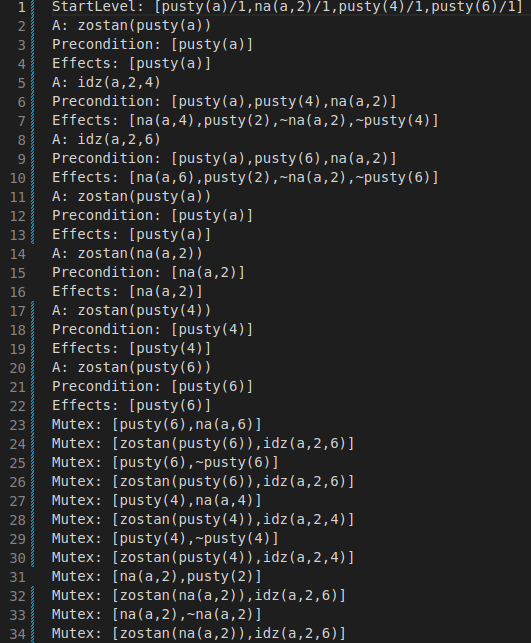
\includegraphics[scale=0.5]{txt_file}
        \centering
        \caption{Urywek przykładowego pliku tekstowego wygenerowanego przez algorytm}
    \end{figure}
    Algorytm na każdym etapie kreowania grafu planującego dokonuje zapisu do pliku tekstowego. Zapisywane są takie informacje jak poziom stanów, 
    akcji czy mutexy. Każda linia pliku rozpoczyna się sygnaturą, po której występuje symbol \textbf{:}, który pełni rolę separatora. 
    Na tej podstawie algorytm dokonuje klasyfikacji informacji występującej po separatorze. 
    Poniżej znajduje się tabela z sygnaturami jak i ich objaśnieniami:
    \begin{table}[H]
        \centering
         \begin{tabular}{||c | c||} 
         \hline
         Sygnatura & Objaśnienie \\ [0.5ex] 
         \hline\hline
         \textit{StartLevel} & Warunki początkowe przedstawionego świata \\ 
         \hline
         \textit{A} &  Obecnie rozpatrywana akcja \\
         \hline
         \textit{Precondition} & Warunki zajścia wyżej wymienionej akcji \\
         \hline
         \textit{Effects} & Efekty wyżej wymienionej akcji \\
         \hline
         \textit{Mutex} & Pary stanów bądź akcji w relacji wykluczającej \\ 
         \hline
         \textit{ActionLevel} & Zbiór wszystkich akcji dla danej warstwy \\ 
         \hline
         \textit{StateLevel} & Zbiór wszystkich stanów dla danej warstwy\\ 
         \hline
         \textit{ChosenActions} & Zbiór akcji wybranych przez planer dla danej warstwy\\ 
         \hline
         \textit{ChosenStates} & Zbiór stanów zdetermionwanych przez wybrane akcje\\ 
         \hline
         \end{tabular}
         \caption{Tabela sygnatur linii w pliku tekstowym}
    \end{table}

    \subsection{Graf pełny}

    \begin{figure}[H]
        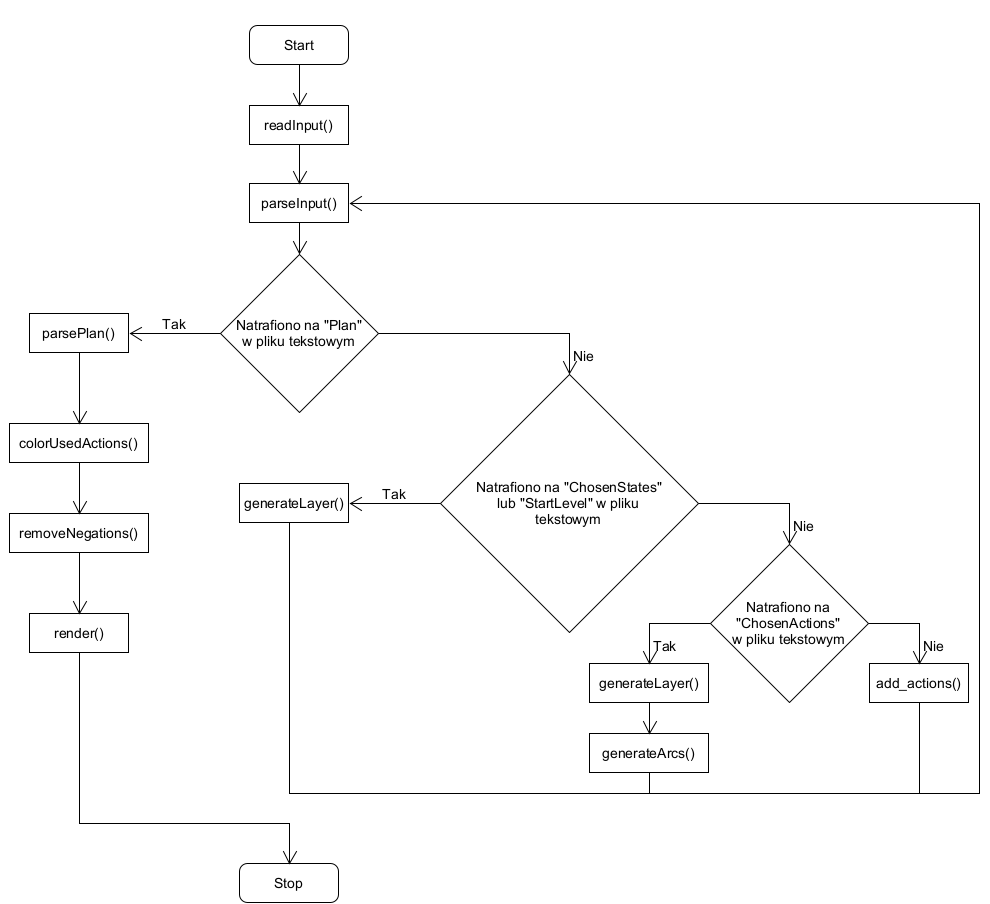
\includegraphics[scale=0.5]{UML_simplified}
        \centering
        \caption{Diagram przepływu dla generowania pojedynczego grafu pełnego}
    \end{figure}

    Na podstawie otrzymanego pliku tekstowego moduł \textit{parsePlanFULL.py}, w którym zaimplementowana została klasa \textit{Graph},
    rozpoczyna generowanie grafu. Pierwszym krokiem jest zainicjalizowanie obiektu klasy \textit{Graph} co jest wykonywane przez warstwę graficzną.
    Następnie przy pomocy metody \textit{run\_all()} dochodzi do uruchomienia procesu generowania grafu. Na powyższym diagramie przepływu należy 
    zauważyć, iż moment oznaczony symbolem \textit{Start} odnosi się do momentu uruchomienia przez warstwę graficzną wyżej wskazanej metody.
    Po uruchomieniu generatora, moduł wczytuje plik by następnie dokonać jego parsowania.

    \subsubsection{Funkcja $parse\_input()$}
    \begin{pseudokod}[H]
        \SetArgSty{normalfont}
        \SetKwFunction{parse}{parse}
        \SetKwFunction{generateLayer}{generateLayer}
        \SetKwFunction{generateArcs}{generateArcs}
        \SetKwFunction{generateMutexArcs}{generateMutexArcs}
        \KwIn{plik tekstowy $Filename$}
        $current\_level\_actions \leftarrow Dict \{\}$ \\
        $prev\_action \leftarrow  String()$ \\
        $mutex\_states \leftarrow List []$ \\
        \ForEach{$linia \in Filename$}{
            $name$, $variables \leftarrow linia$; \\
            $variables \leftarrow parse(variables)$; \\
            \If{$name$ = StartLevel}{
                $generateLayer(variables)$;
            } 
            \If{$name$ = A}{
                $prev\_action \leftarrow variables$; \\
                Dodaj $prev\_action$ jako klucz do słownika $current\_level\_actions$;
            }
            \If{$name$ = Precondition}{
                Dodaj $variables$ jako warunki zajścia w słowniku $current\_level\_actions$ dla $prev\_action$;
            }
            \If{$name$ = Effects}{
                Dodaj $variables$ jako efekty w słowniku $current\_level\_actions$ dla $prev\_action$;
            }
            \If{$name$ = Mutex}{
                Dodaj $variables$ do $mutex\_states$;
            }
            \If{$name$ = ActionLevel}{
                $generateMutexArcs(mutex\_states)$; \\
                $mutex\_states \leftarrow []$; \\\
                $generateLayer(variables)$; \\
            }
            \If{$name$ = StateLevel}{
                $generateArcs(current\_level\_actions)$; \\
                $generateLayer(variables)$; \\
                $current\_level\_actions \leftarrow \{\}$;
            }
            \If{$name$ = Plan}{
                return $variables$;
            }
        }
        \caption{Schemat działania funkcji parse\_input()}
    \end{pseudokod}

    Funkcja w zależności od aktualnej sygnatury zmienia swoje działanie. Należy zauważyć, iż wszystkie akcje, a co za tym idzie ich efekty oraz 
    warunki zajścia są zbierane w strukturze określonej mianem \textbf{Dict}, czyli tablicy asosjacyjnej (inna nazwa: słownik). 
    Dane w tej strukturze są przechowywane w formie par $(klucz,wartość)$. Dokładniej rzecz biorąc, $current\_level\_action$ składa się ze słownika 
    słowników. Kluczem zewnętrznego słownika jest akcja (przykład: $idz(a,1,2)$), nastepnie kluczem wewnętrznego słownika są dwie wartości: 
    \textit{Precondition} oraz \textit{Effects}, do których w formie wartości dodawane są odpowiednio warunki zajścia jak i efekty zgodnie 
    z nomenklaturą STRIPS.
    Dodatkowo funkcja składa się z dodatkowej listy o nazwie $mutex\_states()$, która zbiera wszystkie relacje wzajemnego wykluczania w 
    danej warstwie grafu. 

    Funkcja parsująca $parse()$ jest \textit{wyrażeniem regularnym}, które konwertuje jeden duży ciąg znaków na listę pomniejszych względem 
    separatora przecinka (textit{,}). To co należy zauważyć, to fakt, iż wyrażenie regularne zostało skonstruowane w taki sposób, aby nie 
    dokonywało podziału linii względem przecinków znajdujących się w nawiasach. Gdyby taka funkcjonalność nie została zaimplementowana, napis 
    \textit{idz(a,2,3)} zostałby podzielony na listę napisów: "[idz(a","2","3)]". 

    \begin{listing}[H]
        \begin{minted}{python}
            variables = re.split(',(?![^(]*\\))',variables)
        \end{minted}
    \caption{Implementacja parsowania pliku tekstowego}
    \label{REGEX}
    \end{listing}
    Wynik działania ów parsera dla przykładowego napisu "[pusty(3),na(a,3)]" to ["[pusty(3)","na(a,3)]"].

    Kolejnym krokiem jest uruchomienie funkcji odpowiedzialnych za generowanie grafu w momencie pojawienia się odpowiedniej sygnatury. 
    Ów funkcje to odpowiednio: $generateLayer(), generateArcs()$ oraz $generateMutexArcs()$.

    Metoda $generateLayer()$ ma za zadanie wygenerowanie poziomu stanów na podstawie otrzymanej listy stanów. Robi to, dodając do istniejącej instancji 
    grafu dostarczonej dzięki bibliotece \textbf{graphviz}, kolejnego klastra, który w grafie symbolizowany jest poprzez szarą ramkę.
    \begin{listing}[H]
        \begin{minted}{python}
            def generateLayer(self,name,variables,g,level,type):
            layer_name = 'cluster_' + name
            with g.subgraph(name=layer_name) as layer:
                layer.attr(color='gray')
                layer.attr(label=name)
                for item in variables:
                    layer.node(item+str(level),item, shape=type)
        \end{minted}
    \caption{Implementacja funkcji generateLayer()}
    \end{listing}
    Każdy z klastrów musi posiadać swoje unikalne imię. Generowane jest ono na takiej samej zasadzie jak nazwy poziomy stanów oraz akcji, poprzez 
    konkatenację słów kluczowych oraz wartości iteratora, który symbolizuje aktualną warstwę grafu planującego. 

    Metoda $generateArcs()$ odpowiada za utworzenie krawędzi między stanami a akcjami. Iterując po zbiorze akcji dla danej warstwy łączy warunki 
    zajścia z akcją oraz akcję z jej efektami. W przypadku, gdy nazwa akcji zawiera w sobie frazę \textit{zostań} generowana jest przerywana linia, 
    symbolizująca akcję podtrzymującą. Krawędzie ciągłe charakteryzują się tym, iż strzałka składa się z linii ciągłej. Graf planujący jest 
    grafem acyklicznym skierowany, co powoduje, iż każda z krawędzi zakończona jest strzałką- symbolizuje to skierowaność, którą można
    interpretować jako jednostronne połączenie.

    Metoda $generateMutexArcs()$ odpowiada za utworzenie krawędzi między stanami bądź akcjami, które są ze sobą w relacji wzajemnie wykluczającej. 
    Efektem działania tej funkcji jest niebieska, przerywana linia łącząca w pary odpowiednie obiekty grafu.

    Każdy plik kończy się linią zawierającą plan. Jeśli funkcja $parse\_input()$ natrafi na rzeczoną linię, parsuje ją i zwraca jej zawartość 
    jako utworzony przez algorytm \textbf{plan}.

    \subsubsection{Oznaczenie planu na grafie}

    Po zakończeniu działania metody $parse\_input()$ główna jednostka sterująca przepływem działania generatora grafu przechodzi do funkcji, której 
    zadaniem jest rozbicie planu na warstwy oraz akcje, która w danej warstwie należy wykonać, aby uzyskać wskazany cel. Realizowane jest to przy 
    pomocy funkcji $parsePlan()$ oraz wyrażenia regularnego (kod źródłowy \ref{REGEX}). Dodatkowo w celu wyelimiowania nieczytelnych dla człowieka informacji z 
    listy akcji elimionwane są akcje podtrzymujące (w odróżnieniu od algorytmu człowiek wie, iż brak któreś z komponentów w 
    akcjach danej warstwy skutkuje brakiem zmiany jego stanu). Wykonywane jest to za pomocą metody $planWoPersist$, która eliminuje wszystkie 
    elementy z planu zawierające frazę \textit{zostań}. 
    Następnie program przechodzi do ostatniego etapu: zaznaczania akcji wchodzących w skład planu poprzez zmianę kolory na czerwonych wszystkich 
    krawędzi, które z ów akcją są połączone. Implementacja tego mechanizmu została wykonana w ramach funkcji $colorUsedActions()$ i w swoim działaniu 
    jest bardzo prosta- wyszukuje warunki zajścia, jak i efekty dla wskazanej akcji i zmienia kolory krawędzi, które je łączą. Ważnym jest, iż ze 
    względu na odfiltrowanie akcji podtrzymujących, barwa ich krawędzi nie zostanie zmieniona w wygenerowanym grafie. 

    Gdy wszystkie krawędzie zmieniające świat zgodnie z zawartością planu zmienią swój kolor, program wykonuje procedurę $render()$, która 
    generuje graf o zadanych własnościach. Procedura $render()$ pochodzi bezpośrednio z biblioteki \textit{graphviz}.

    Efektem działania programu jest następujący graf pełny:

    \begin{figure}[H]
        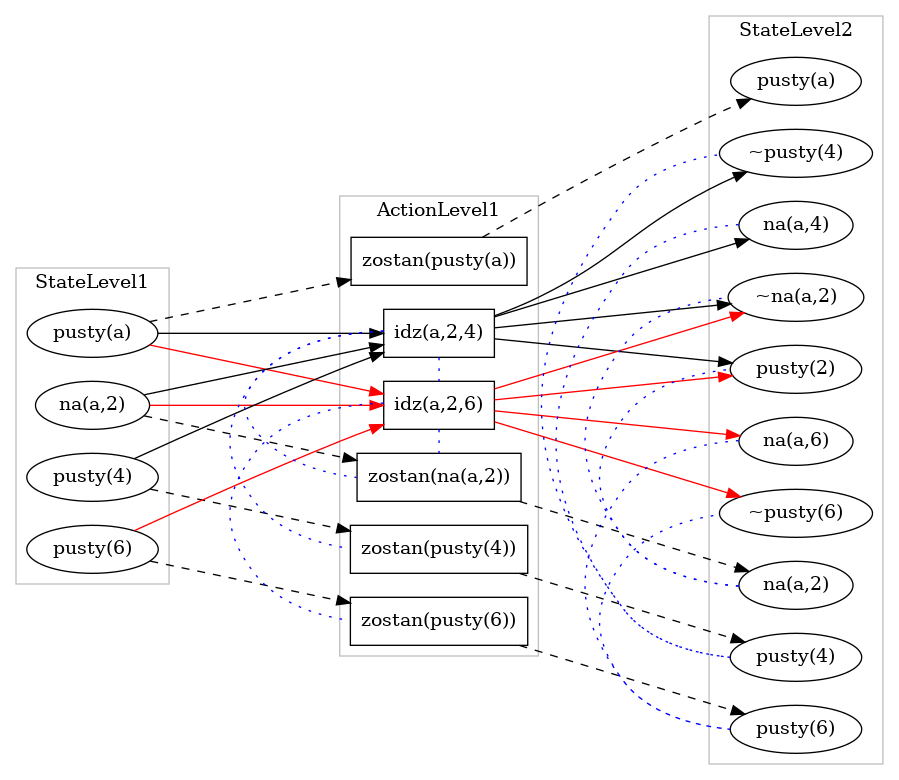
\includegraphics[scale=0.25]{GrafPelny1}
        \centering
        \caption{Przykład grafu pełnego dla prostego przypadku}
    \end{figure}
    Jednakże ze względu na liczbę stanów, jakie mogą wchodzić w skład danego poziomu stanów czy akcji oraz na liczbę krawędzi między stanami, graf 
    pełny bardzo szybko staje się nieczytelny dla człowieka, co przedstawia następująca ilustracja:
    \begin{figure}[H]
        \includegraphics[scale=0.02]{GrafPelny2}
        \centering
        \caption{Przykład grafu pełnego dla złożonego przypadku}
    \end{figure}
    Z tego powodu utworzono dodatkową klasę, która generuje podgraf grafu pełnego, który zawieraja jedynie istotne z perspektywy człowieka informacje.
    Taki graf w dalszej części pracy będzie nosił miano \textit{grafu prostego}.

    \subsection{Graf prosty}

    Graf prosty tworzony jest na podstawie grafu pełnego z wyelimiowaniem pewnych elementów w celu zwiększenia czytelności prezentowanych danych.
    \begin{figure}[H]
        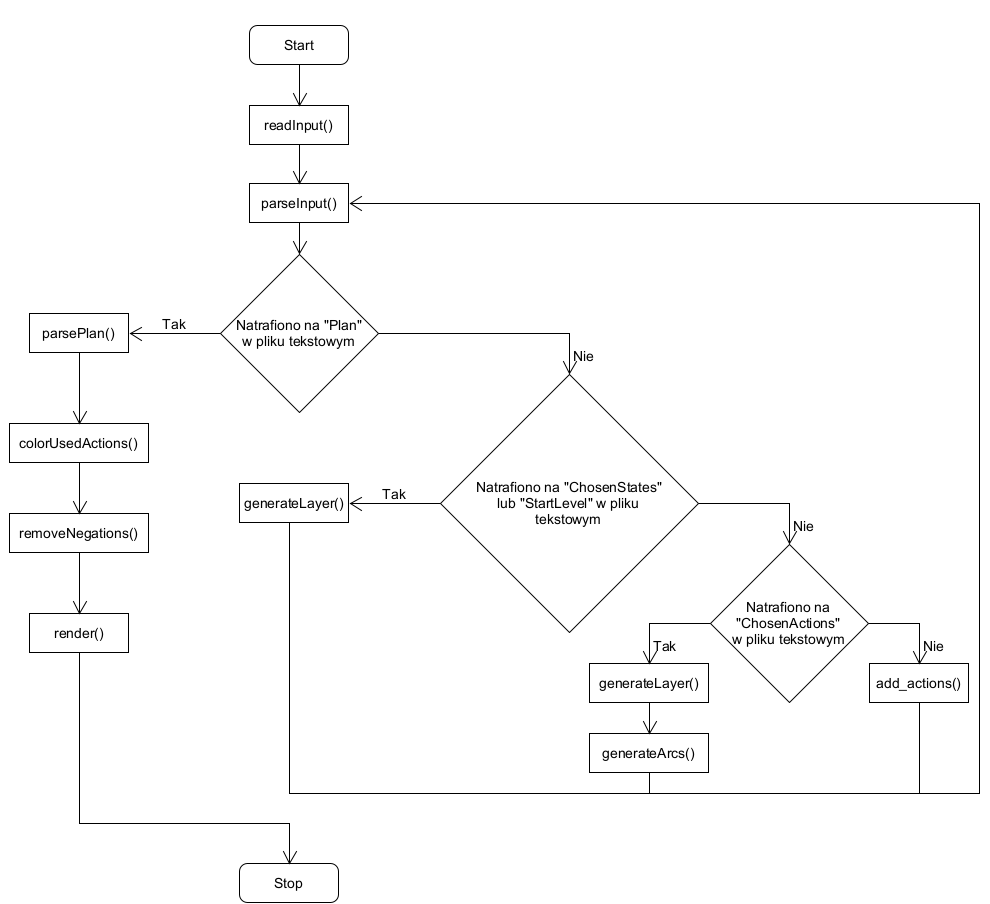
\includegraphics[scale=0.5]{UML_simplified}
        \centering
        \caption{Diagram przepływu dla generowania pojedynczego grafu prostego}
    \end{figure}
    Większość znajdujących się na diagramie funkcji, których implementację można znaleźć w pliku \textit{parseplanSIMPLFIED.py} w ramach klasy 
    \textit{SimplifiedGraph}, jest identyczna względem grafu prostego. Główne różnice występują w mechanizmie parsowania planu, ze względu na obiekty, 
    które zostały wyeliminowane na rzecz czytelności grafu. Graf prosty składa się z:
    \begin{enumerate}
        \item Stanu dla każdego obiektu, które są prawdziwe w danej warstwie
        \item Akcji dla każdego obiektu w danej warstwie
        \item Specjalnego oznaczenia wykorzystywanych akcji aktywnych wraz z oznaczeniem krawędzi, rodem z grafu pełnego
    \end{enumerate}
    Różnica względem grafu pełnego jest brak generowania mutex'ów, hipotetycznych stanów, w których dany obiekt mógłby się znaleźć oraz efektów usuwających.
    
    Efektem działania programu jest następujący graf:
    \begin{figure}[H]
        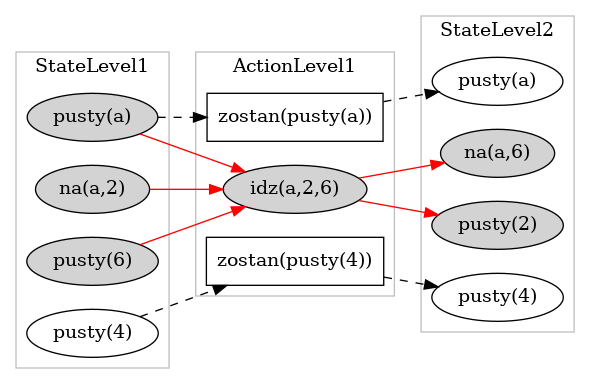
\includegraphics[scale=0.5]{GrafProsty1}
        \centering
        \caption{Przykład grafu prostego dla prostego przypadku}
    \end{figure}
    Dla przypadku złożonego czytelność planu wzrosła diametralnie przy drobnej utracie wiedzy o planie. Jednakże, z perspektywy człowieka wykonujacego 
    wskazany plan na podstawie grafu, występowanie hipotetycznych stanów jest całkowicie zbędny, istnienie negatywnych efektów funkcji jest dla 
    człowieka naturalnym do wydedukowania, a brak oznaczonych mutex'ów wynika z faktu, iż w skład grafu wchodzą jedynie akcje, 
    które należy wykonać aby otrzymać dany cel. Poniższy przykład przedstawia graf dla złożonego przypadku:
    \begin{figure}[H]
        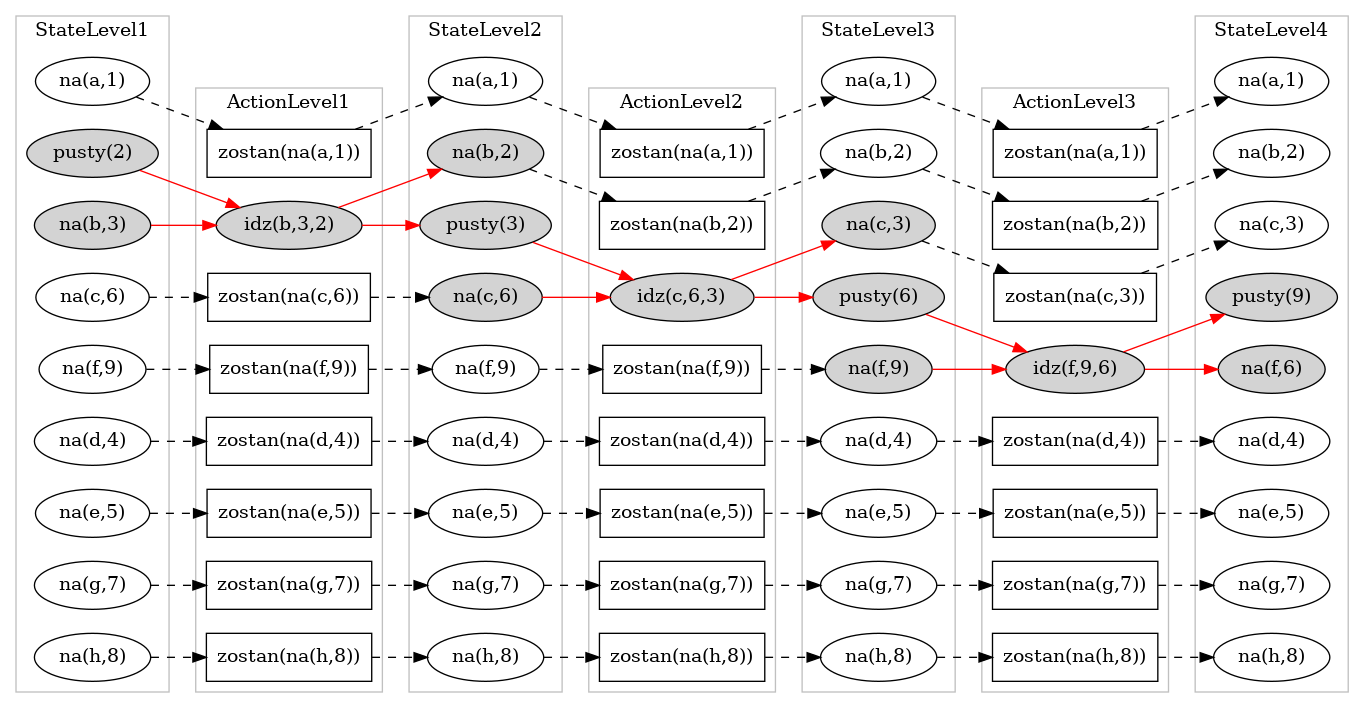
\includegraphics[scale=0.25]{GrafProsty2}
        \centering
        \caption{Przykład grafu pełnego dla złożonego przypadku}
    \end{figure}

\section{Interfejs użytkownika}
    Interfejs użytkownika wykonany w języku \textbf{python} stanowi spoiwo, łącząc w sobie wygenerowany plan przez algorytm oraz wygenerowane grafy przez 
    odpowiedni moduł. Poniższa ilustacja przedstawia w sposób ogólny diagram przepływu w trakcie obsługi programu przez użytkownika: \\
    //Tutaj rysunek + opis ważniejszych funkcji

    Po uruchomieniu pliku \textit{gui.py} (preferowana ścieżka uruchomienia to linia komend, przy użyciu komendy python3 gui.py).
    pojawia się następujace okienko:
    \begin{figure}[H]
        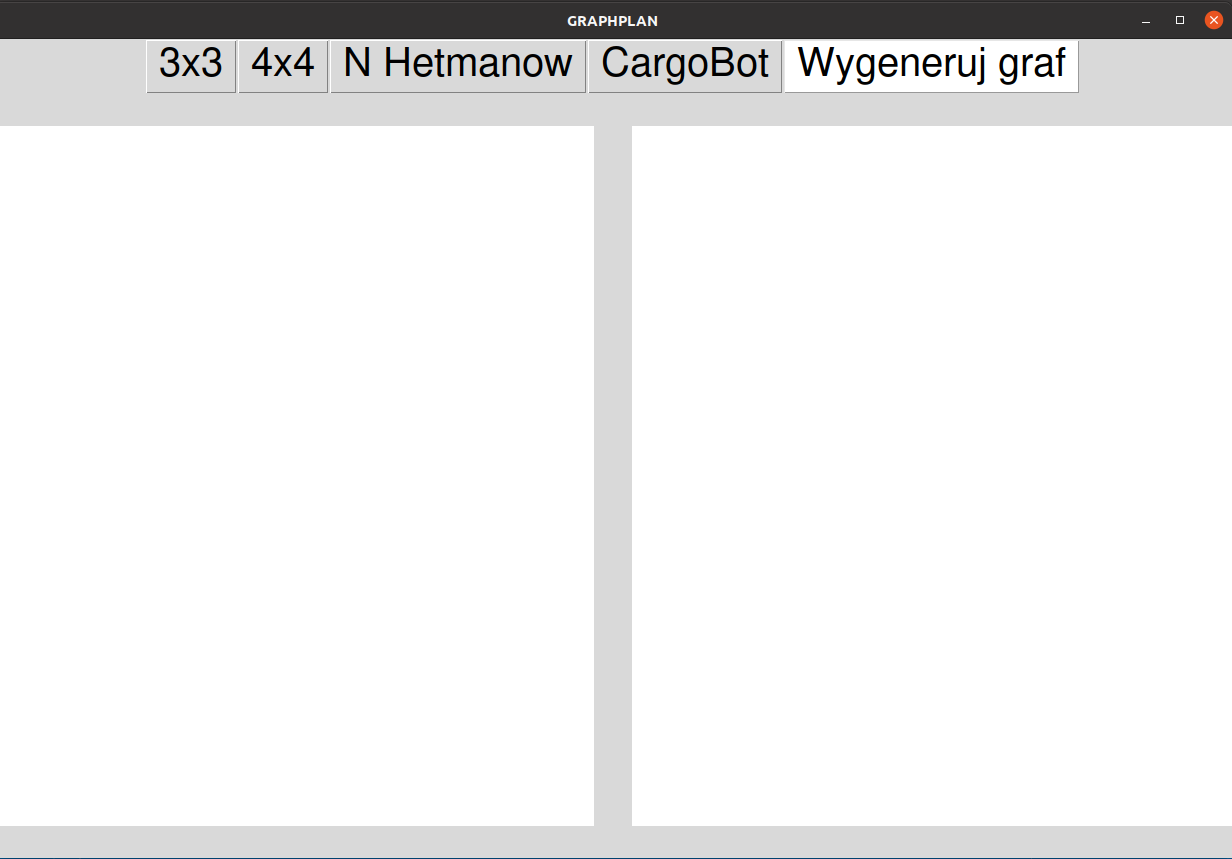
\includegraphics[scale=0.3]{GUIMain}
        \centering
        \caption{Okno startowe programu}
    \end{figure}

    W górnym panelu znajdują się przyciski, które odpowiadają odpowiednim światom. Sygnatury znajdujące się na przyciskach zostały 
    dokładniej przedstawione w sekcji odpowiedzialnej za testy algorytmu (3x3 i 4x4: \ref{15Test}, CargoBOT: \ref{CargoBotTest}, 
    Osiem Hetmanów: \ref{OsiemHetmanowTest}). Po wybraniu jednej z opcji, użytkownik zostaje przeniesiony w obszar roboczy związany z wybranym
    otoczeniem.

    \begin{figure}[H]
        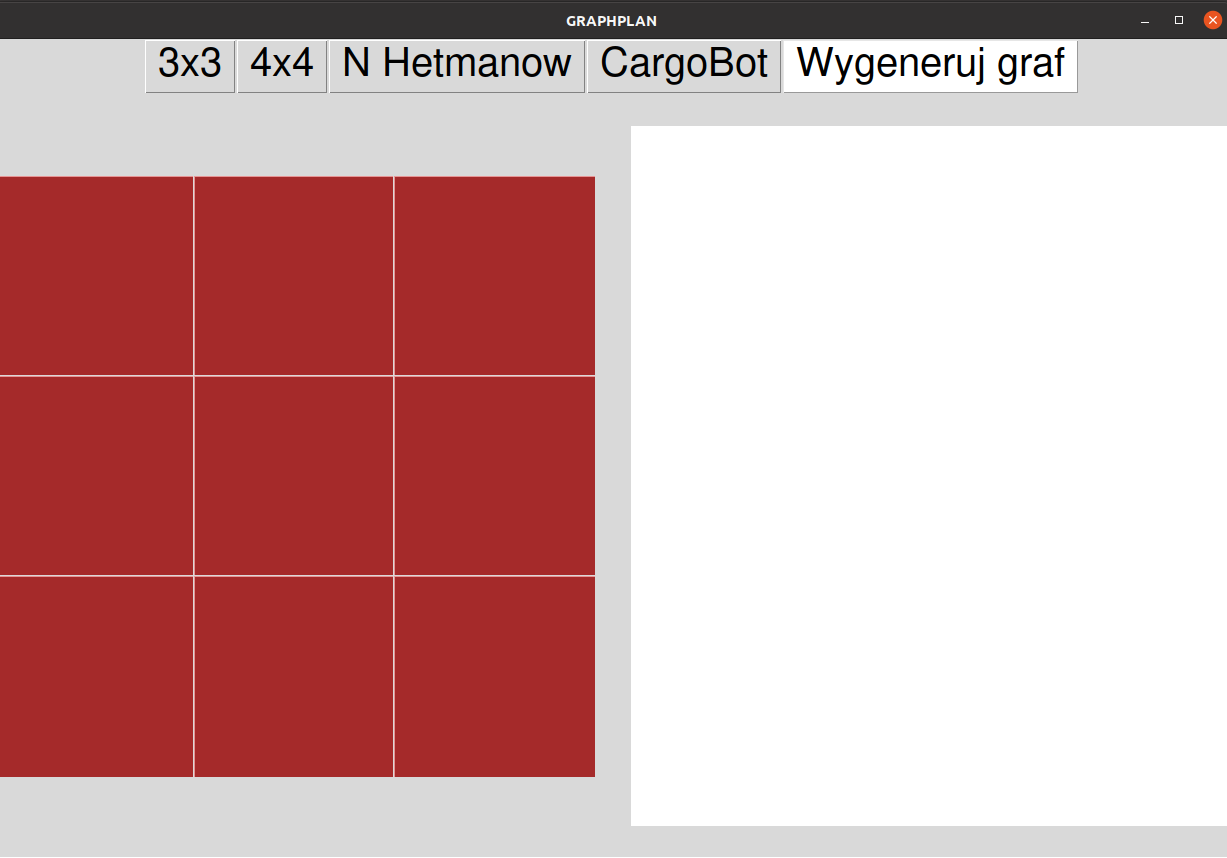
\includegraphics[scale=0.3]{GUI3x3Empty}
        \centering
        \caption{Widok po wybraniu opcji "3x3"}
    \end{figure}

    \begin{figure}[H]
        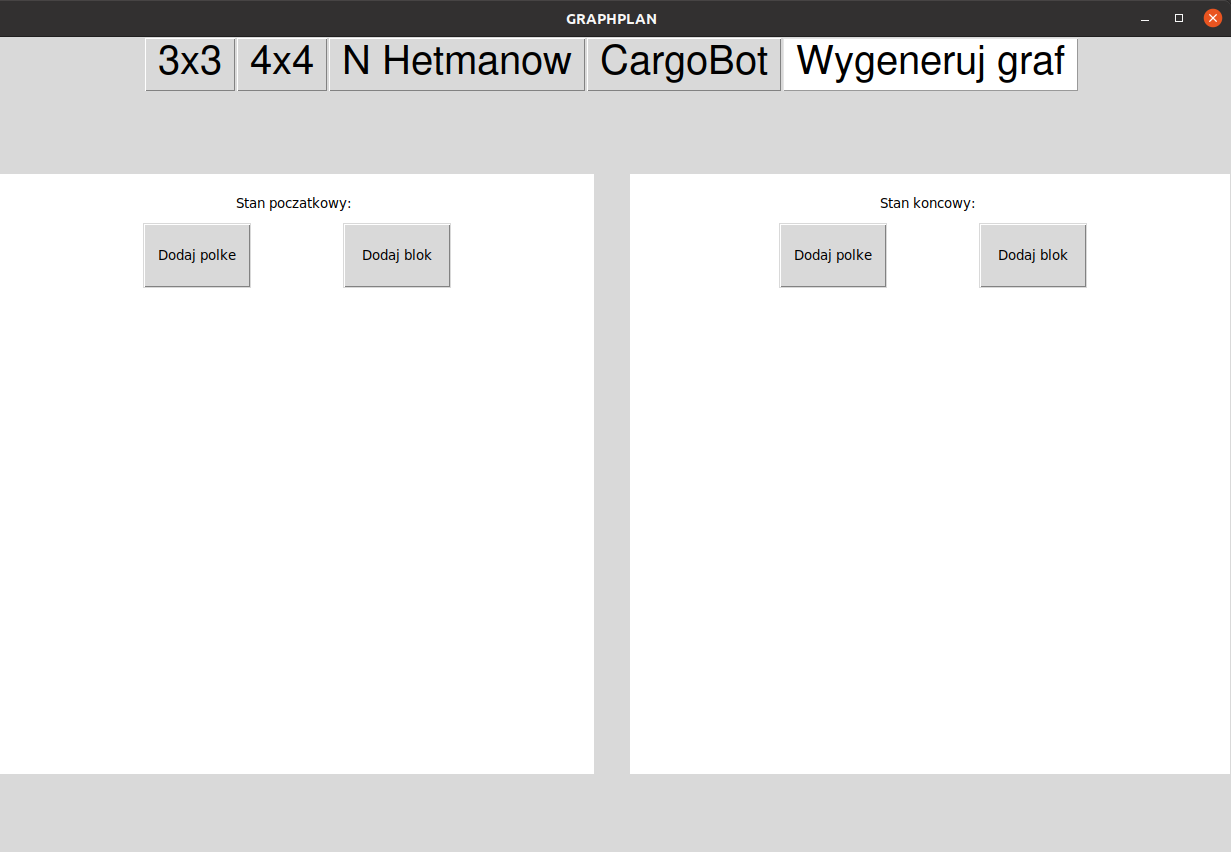
\includegraphics[scale=0.3]{CargoBOTEmpty}
        \centering
        \caption{Widok po wybraniu opcji CargoBOT}
    \end{figure}

    Powyższe ilustracje przedstawiają dwa typy światów: jeden, w którym cel jest z góry ustalony, więc użytkownik dysponuje jedynie lewym panelem w 
    celu określenia stanu początkowego, oraz drugi, w którym użytkownik samodzielnie definiuje warunki początkowe jak i wymagany cel.

    Po zdefiniowniu odpowiedniego stanu początkowego, przy pomocy przycisku "Wygeneruj graf" dokonywane jest generowanie grafu wraz z graficznym 
    przedstawieniem planu z podziałem na kroki:

    \begin{figure}[H]
        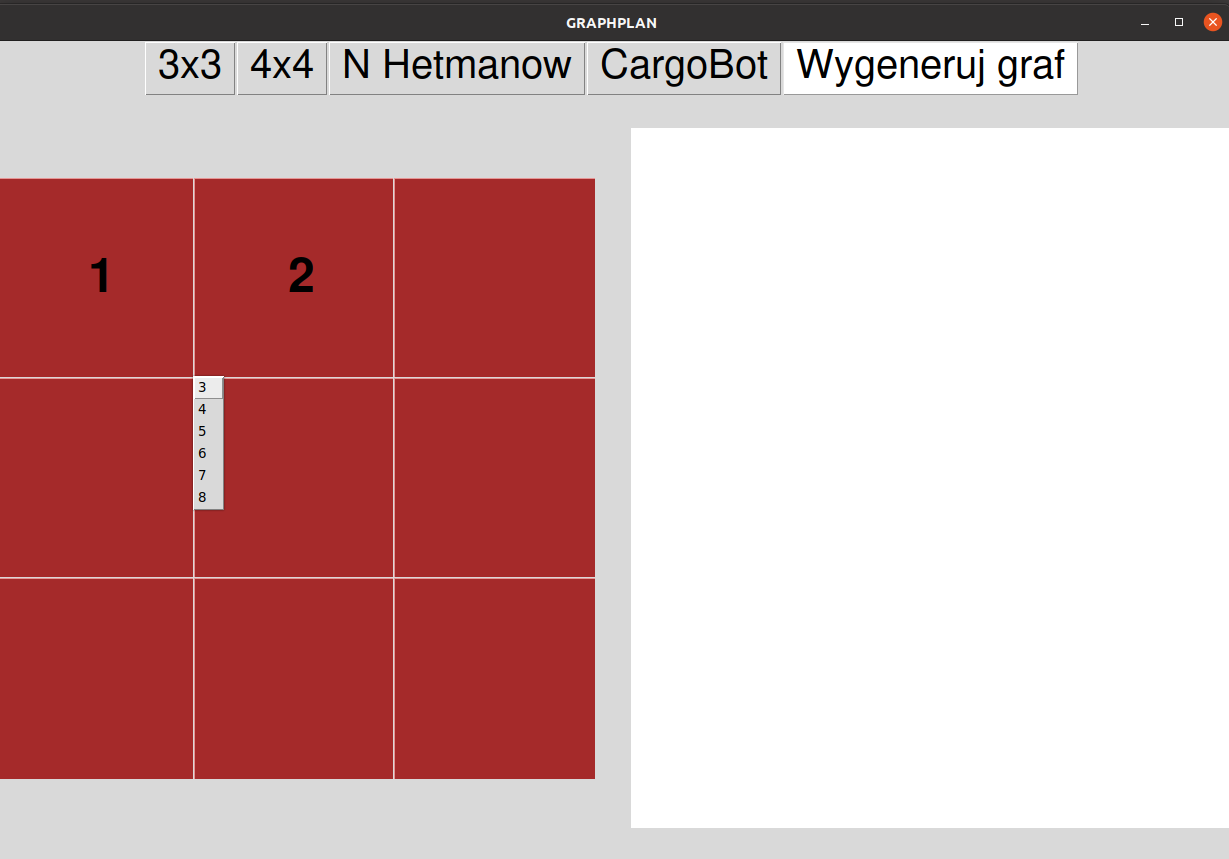
\includegraphics[scale=0.3]{GUI3x3Wypelnianie}
        \centering
        \caption{Proces definiowania świata}
    \end{figure}

    \begin{figure}[H]
        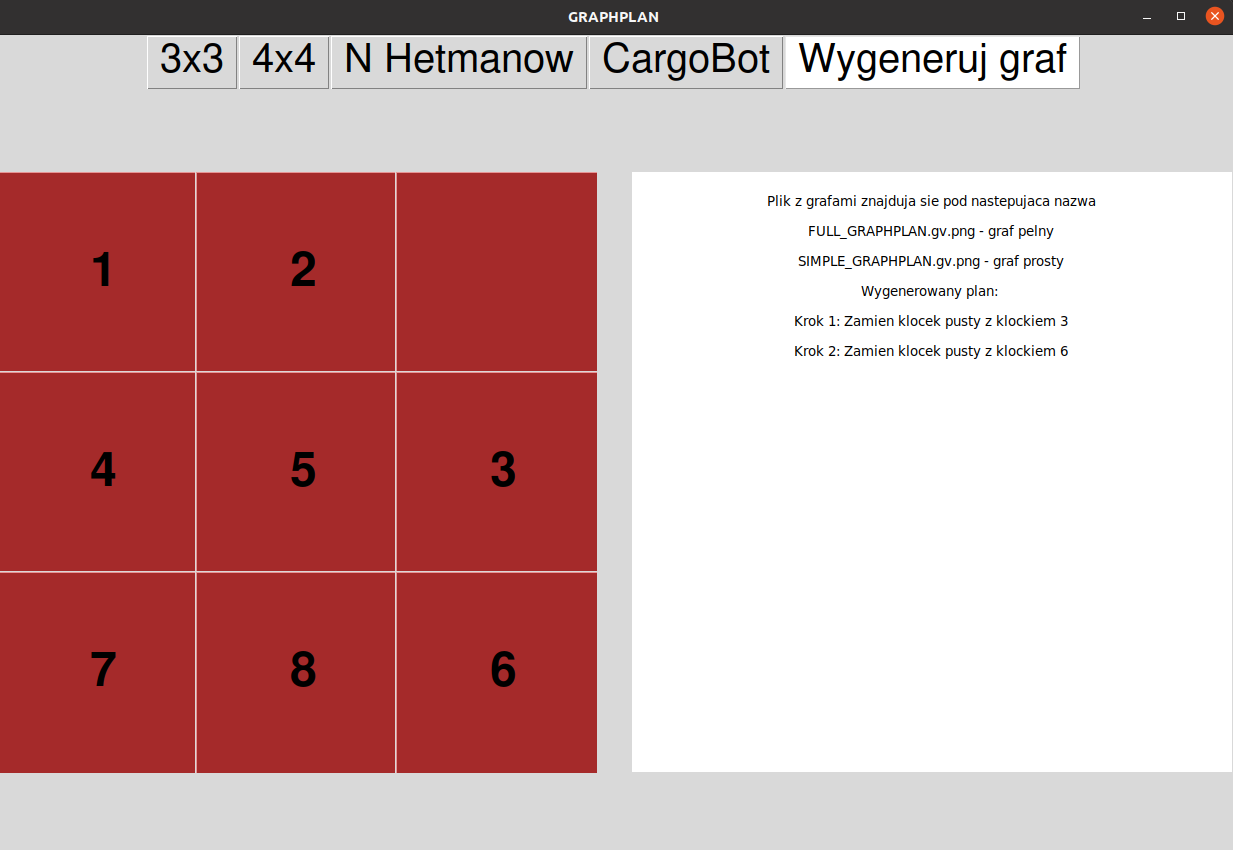
\includegraphics[scale=0.3]{GUI3x3Wynik}
        \centering
        \caption{Stan po wygenerowaniu planu}
    \end{figure}

    Odpowiednie grafy generowane są w folderze \texttt{graphs} o nazwach wskazanych przez okno wynikowe.
\section{Uruchomienie algorytmu z linii komend}
    \label{CommandLine}
    Zalecanym sposobem uruchomienia algorytmu jest wykorzystanie specjalnie przygotowanego programu graficznego, jednakże implementacja zezwala na 
    wykonywanie planów z linii komend. Ów funkcjonalność została wykorzystana między innymi w testach, których opis można znaleźć w ostatnim rozdziale pracy.
    Aby uruchomić program z linii komend należy wprowadzić następującą komendę \textit{swipl}, która uruchomi środowisko języka programowania PROLOG.
    Jeśli użytkownik posiada inną implementację języka, zobowiązany jest do samodzielnego zapoznaia się ze sposobem uruchomienia interaktywnego 
    środowiska wewnątrz terminala (więcej w sekcji \ref{SWI-PROLOGRozdzial})
    \subsubsection{Definicje świata}
    Przeglądając plik \textit{graphplan.pl} można zauważyć, iż jest on pozbawiony podstawowych definicji wchodzących w skład opisu STRIPS. Wynika 
    to z faktu, iż uruchamiając program przy pomocy graficznego interfejsu, przy wyborze odpowiedniego świata, 
    generowane są wszystkie niezbędne relacje i dołączane do środowiska, w którym znajduje się kod źródłowy algorytmu.
    Użytkownik samodzielnie musi zadbać o wprowadzenie odpowiednich informacji o świecie. Może to wykonać w następujący sposób:
    \begin{itemize}
        \item Przed wczytaniem zawartości pliku \textit{graphplan.pl} do środowiska interaktywnego może "dokleić" własne linijki kodu 
        zawierające opis świata, w którym chciałby wygenerować odpowiedni plan. Doklejanie należy wykonać po ostatniej komendzie zaczynającej 
        się słowem \textit{dynamic}. Dodatkowo, definiując własne relacje, których nazwy nie zawierają się w sekcji dynamic, użytkownik 
        zobowiązany jest do jej uzupełnienia zgodnie z wzorcem, który znajduje się w pliku źródłowym
        \item Po wczytaniu zawartości pliku \textit{graphplan.pl} użytkownik może manipulować relacjami w świecie poprzez wykorzystywanie 
        predykatów $assert/1$ bądź $retract/1$. 
    \end{itemize}
    Wczytywanie pliku w środwisku interaktywny SWI-PROLOG można wykonać na dwa sposoby, poprzez zastosowanie nawiasów kwadratowych, wewnątrz których 
    znajduje się nazwa plik ($[graphplan].$), bądź przy użyciu predykatu $consult/1$. Oba sposoby są sobie równoważne. Opis wczytania pliku zakłada,
    iż środowisko interkatywne zostało uruchomione w tym samym katalogu, w którym znajduje się kod źródłowy algorytmu.
    \subsubsection{Uruchomienie algorytmu}
    Zakładając poprawność definicji świata przez użytkownika należy zaopatrzyć algorytm w dwa istotne aspekty: stan początkowy oraz stan końcowy. 
    Stan początkowy wprowadzany jest przy pomocy predykatu $inital\_state/1$, który przyjmuje listę stanów prawdziwych przed rozpoczęciem działań.
    Następnie należy wywołać procedurę $call\_plan/2$ według następującego schematu 
    \begin{equation}
        call\_plan(A,Plan).
    \end{equation}
    gdzie A oznacza listę stanów docelowych.
    Przykładowe uruchomienie algorytmu z poziomu linii komend:

    \begin{figure}[H]
        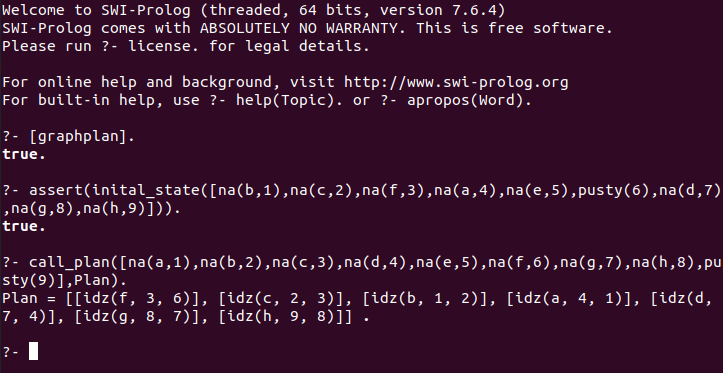
\includegraphics[scale=0.5]{LiniaKomendWywolanie}
        \centering
        \caption{Zrzut ekranu prezentujący przykładowe uruchomienie algorytmu z linii komend}
    \end{figure}

    W pliku \textit{worlds.pl} znajdują się definicje światów wykorzystywanych w ramach badań. Każdy ze światów odzielony jest komentarzem 
    jednolinijkowym wraz z oznaczeniem świata (np. CargoBOT). Kod znajdujący się między sygnaturami komentarza wielolinijkowego przedstawia 
    definicję wskazanego świata.
    Dodatkowo każdy ze światów zawiera kilka przykładów, aby oswoić użytkownika ze specyficznym mechanizmem wprowadzania danych 
    z poziomu linii komend.

